% \cleardoublepage
% \chapter*{Introduction}
% \markboth{Introduction}{Introduction}
% \addcontentsline{toc}{chapter}{Introduction}

\chapter{Introduction}

\section{Problem and Motivation}

Suppose we are given samples of data say $X$ and $Y$, s.t.

\begin{align*}
    X = x_1, ..., x_n  \\
    Y = y_1, ..., y_n 
\end{align*}

For example, we may be measuring the blood pressure and heart rate of Alice at time $k$, 
say $x_k$ and $y_k$ respectively. Further, suppose we are unaware of her context, for example,
Bob hacked into Alice's apple watch and so can only read $X$ and $Y$ -- but he has no idea of 
anything she might be up to.

Bob then observes the following trend:

\begin{figure}[H]
    \centering
    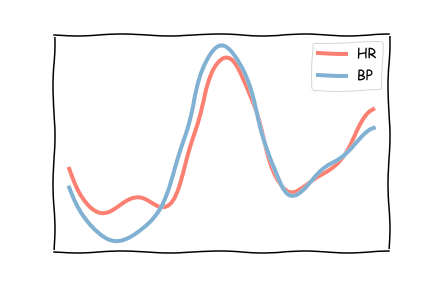
\includegraphics[width=.45\textwidth]{correlated_hr.png}
    \caption{Heart rate (HR) and Blood pressure (BP) of Alice.}
\end{figure}

Bob, having studied data science, is well aware of the fallacy of the law of small numbers\footnote{
    The law of small numbers is the error of concluding too much from too few data. 
}. He therefore checks again the data the next day at a slightly different time. He again observes 
a similar trend, and is now more confident in the existance of a causal relation -- having neglected biology as 
being beneath him -- and makes the conjecture that either blood pressure causes heart rate, or 
perhaps the other way around. 

Given this strong correlation, Bob asserts that he may either model $X$ as a function of $Y$ or the other way 
around. He proceeds to find some $f$ s.t. $f(X) \approx Y$. The next day, to his dismay, he notices that his
model has terrible performance when evaluated on new data. He then proceeds to see what is going on, and 
observes the following:

\begin{figure}[H]
    \centering
    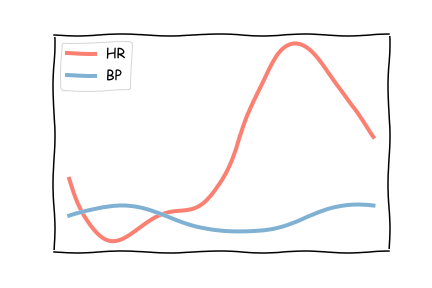
\includegraphics[width=.45\textwidth]{uncorrelated_hr.png}
    \caption{Heart rate (HR) and Blood pressure (BP) of Alice.}
\end{figure}

As it turns out, in the last few days, Alice was working hard on finishing her thesis and the deadline had been 
the previous day. But how, Bob wondered, could this have changed the relationship between BP and HR? 
Finally, admitting to himself that machine learning alone is not enough to understand the world; 
Bob spends some time learning about the heart. It turns out, that fear triggers a "flight or fight"
response that increases both the heart rate and blood pressure; Interestingly your heart rate and blood pressure 
won’t always rise and fall in sync.

So what did Bob learn\footnote{
    Note that heart rate and blood pressure are intimately linked, and the story between them is more complicated.
    The plots were randomly generated using a gaussian process, however they do resemble some real examples that 
    can be found in google images.
}?

\begin{enumerate}
    \item When we train a model with some data, when we use it on some newly aquired data, we might
    face a \textbf{covariate-shift} -- that is, the distribution might change due to the context changing.
    \item When we see correlation it might be spurious due to a \textbf{confounder} -- fear was the \textbf{confounder} 
    of the heart rate and blood pressure.
    \item His degree in Data Science is worth less than he thought; \textbf{machine learning is in fact not 
    a panacea}, contrary to common culture. However, applied with domain knowledge and causal reasoning
    it may very useful. 
\end{enumerate}

If Bob was able to incorporate these notions into his machine learning models, then he might have been more
robust to the covariate-shift. To give a more concrete example, there is a "neural net tank urban legend"\footnote{
    More about this story here: https://www.gwern.net/Tanks.
}
, where a neural network accuratly predicts if there is a tank or not in an image, but it turns out it uses the 
weather as a predictor. From this it is clear that the model will preform badly under covariate shift, and indeed
it makes the case that incorporating causality to a model should make it more robust as Scholkopf 
argues (\cite{scholkopf2019causality}).

As for confounders, it is impossible to say anything in general\footnote{
    For most of the 20th century, a huge debate took place to determine the question of whether or not 
    smoking caused cancer. A clever argument against a causal relation was that there existed a gene that 
    made a person both want to smoke and more prone to cancer; even the father of modern statistics
    himself thought this explanation more plausible (For a good read on how science is and was used 
    for wrong see the excellent book \cite{NaomiMerchants}).
    
}. We must therefore specify a causal model, and
then see what gurantees we can give under what assumptions. Even in the absence of confounders it is highly 
non trivial to determine causality.

As this simple example illustrates, causality is related to many interesting questions; perhaps, one of the most 
simple questions we can ask -- and the one that we will explore -- is, given that either X causes Y, or Y causes X
(we assume no confounders) then, when 
can we predict the direction of causality? If yes, how? 

In the figure bellow (figure \ref{fig:simple_bivariate_example}) can you tell if $X$ causes $Y$? Or perhaps
it is the other way around? In fact\footnote{ We model $y = f(x) + n$,  where x is exponential distribution, and n 
normaly, both independent from each other; $f$ is a non-linear function. This kind of set up is known as an 
additive model and it will be a central object of study.} $X$ causes $Y$, and we will show algorithms that 
can accuretly predict causality in such settings with as few as 75 samples. 

\begin{figure}[H]
    \centering
    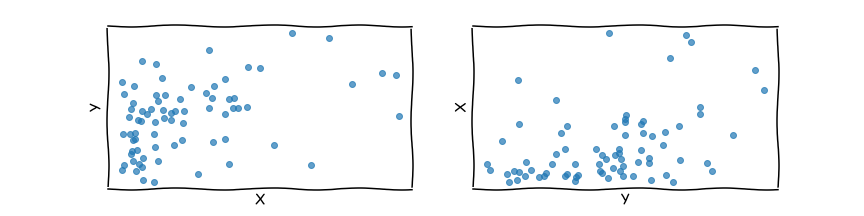
\includegraphics[width=1\textwidth]{bivariate_causal_example.png}
    \caption{75 samples of data $X$, $Y$.  }
    \label{fig:simple_bivariate_example}
\end{figure}

\section{Causality}

We have seen in the introduction that determining and understanding causality may indeed be useful; 
but what exactly is causality? When we say $X$ causes $Y$ i.e. $X \rightarrow Y$, we have an intuitive
idea of what it means; but how should we formalise it?

Suppose that we are given two random variable $X$, $Y$ with joint distribution $\Prob (x, y)$. Intuitively we 
would say that $X \rightarrow Y$, if we intervene in $X$ and then see an effect $Y$. In particular
we will denote $\operatorname{do}(x)$ -- short for $\operatorname{do}(X = x)$ -- as an intervention
that forces the variable $X$ to have the value $x$, and leaves the rest of the system untouched. 
Following the convention inspired by \cite{pearl2000causality}, 
we define the resulting distribution as $\Prob_{Y|do(x)}$.

In supervised learning the goal is often to estimate $p_{y|x}$; while it is tempting to say that this is the 
same as $p_{y|do(x)}$, they may in fact be very different. Suppose $x$ is 1 if a person smokes and 0 otherwise, 
similarly let $y$ be 1 if a person has cancer and 0 otherwise. If we then ran immoral 
\textbf{randmoized trials}\footnote{The power of randmoized trials is that they average out potential confounder 
-- e.g. a gene that causes both an inclination to smoke and cancer. This is also knowm as A/B testing and is 
essential to determine if a new medicine has the desired effect and that a new UI might maximise user addicton 
to an app.} and forced a subset of the population at random to smoke, then we could estimate $p_{y|do(x)}$. 
If it turned out that $p_{y|do(x)} \approxeq p_{y|x}$ then this would be very strong evidence that indeed 
smoking caused cancer.

This motivates the following definition

\begin{definition}
    We say that $X$ \textbf{causes} $Y$ if $p_{y|do(x)} \neq p_{y|do(x^\prime)}$ for some
    $x, x^\prime$
\end{definition}


Borrowing from probability, it might be tempting to say something like 

$$
    p_{y|x}
$$

From our own lives, we know that it is by intervening in systems that we infere causal directions. 


\section{Proposed Methods}

We propose two methods to deal with the ANM -- one less practical, but with a nice theoretical
analysis; and another more practical, but perhaps with a less pleasing analysis. However both
are based on a first principle approach with known asymptotics in mind.

We note that in the analysis / procedure we split the data in 2, first to train the model, and
then to perform the score computation - Need to expand on this

Will be easier to do once they are finished.


\section{Outline}

The thesis is divided in two parts, 

background etc blup blue die blah blu

Do once finished, but main idea

Theory and background material

Methods

Experiments